%============================================================
%  ClipMind — Chat with YouTube Lectures : Project Report
%  Compile with pdfLaTeX (Overleaf-ready). Recompile once;
%  the table of contents resolves automatically.
%  >>> On the title block, fill [Your Name] and [Your Roll Number].
%  >>> Change the course code / degree / institute if yours differ.
%============================================================
\documentclass[11pt,a4paper]{article}

\usepackage[utf8]{inputenc}
\usepackage[T1]{fontenc}
\usepackage[a4paper,margin=1in]{geometry}
\usepackage{graphicx}
\usepackage{xcolor}
\usepackage{booktabs}
\usepackage{tabularx}
\usepackage{enumitem}
\usepackage{listings}
\usepackage{tikz}
\usetikzlibrary{positioning, arrows.meta}
\usepackage[hidelinks]{hyperref}
\hypersetup{colorlinks=true, linkcolor=black, urlcolor=blue!60!black, citecolor=black}

%------------------ colours & code style ------------------
\definecolor{codebg}{RGB}{245,246,250}
\definecolor{codekw}{RGB}{200,40,90}
\definecolor{codestr}{RGB}{22,140,90}
\definecolor{codecmt}{RGB}{130,135,150}
\definecolor{accent}{RGB}{220,50,80}

\lstset{
  backgroundcolor=\color{codebg},
  basicstyle=\ttfamily\footnotesize,
  keywordstyle=\color{codekw}\bfseries,
  stringstyle=\color{codestr},
  commentstyle=\color{codecmt}\itshape,
  breaklines=true,
  frame=single,
  rulecolor=\color{gray!30},
  numbers=left,
  numberstyle=\tiny\color{gray},
  numbersep=8pt,
  showstringspaces=false,
  tabsize=2,
  captionpos=b,
  xleftmargin=16pt,
}

\newcommand{\code}[1]{\texttt{#1}}

\begin{document}

%====================== TITLE BLOCK (IIT-G term-project style) ======================
\begin{center}
  {\LARGE \textbf{ClipMind: A Source-Grounded Conversational\\[2pt]
  Assistant for Video Lectures}}\\[1.1em]
  {\large \textit{[Your Name] ([Your Roll Number])}}\\[0.45em]
  {\normalsize Term Project Report (DA 377)}\\[1.2em]
  {\normalsize B.Sc. (Hons) Data Science and Artificial Intelligence}\\[0.25em]
  {\normalsize Indian Institute of Technology Guwahati, India}
\end{center}
\vspace{1.4em}

%====================== ABSTRACT ======================
\begin{abstract}
\noindent
\textbf{ClipMind} turns any YouTube lecture into an interactive, source-grounded study
assistant. Given a video link, the system obtains a time-stamped transcript (from the
video's captions when available, otherwise by automatic speech recognition), indexes it
using a Retrieval-Augmented Generation (RAG) pipeline, and then lets the user
\emph{chat with the video} and generate a summary, automatic chapters, study notes,
quizzes, keywords and named entities. Crucially, every answer is \emph{grounded in the
transcript} and linked to the exact moment in the video: clicking a cited timestamp
seeks the embedded player to that point. The application is built as a FastAPI backend
and a React single-page frontend. Language understanding is provided by a Large Language
Model served through Groq, retrieval uses Sentence-Transformers embeddings with a FAISS
vector index, and speech recognition uses Whisper. The design is provider-agnostic and
can be reconfigured to use Gemini, OpenAI or a local model without code changes.
\end{abstract}

\newpage
\tableofcontents
\newpage

%====================== INTRODUCTION ======================
\section{Introduction}

\subsection{Overview}
Lectures and talks are increasingly consumed as long online videos. While rich in
content, they are difficult to search, review and study: finding where a specific
concept is explained, or revising a one-hour lecture before an exam, is slow and tedious.
ClipMind addresses this by making a video lecture \emph{queryable} --- a learner can ask
questions in natural language and receive concise, trustworthy answers that point back to
the exact moment in the video.

\subsection{Problem Statement}
To design and build a web application that converts a YouTube lecture into a
source-grounded knowledge base, enabling natural-language question answering and the
automatic generation of study material (summary, chapters, notes, quiz, etc.), with every
answer traceable to a timestamp in the original video.

\subsection{Objectives}
\begin{itemize}[leftmargin=1.4em]
  \item Obtain a time-stamped transcript of any YouTube video: prefer the existing
        captions (fast), and fall back to automatic speech recognition when none exist.
  \item Build a RAG pipeline over the transcript so that questions are answered using
        only the relevant portions of the lecture (grounded, not hallucinated).
  \item Provide \textbf{timestamp citations}: answers reference the moments they rely on,
        and those references are clickable and seek the embedded player.
  \item Generate study aids from the transcript: summary, automatic chapters, notes,
        multiple-choice quiz, keywords and named entities.
  \item Keep the system fast and inexpensive to run.
\end{itemize}

\subsection{Scope}
The current version processes one video per session and stores the resulting index in
server memory for the duration of that session. It focuses on the transcription,
retrieval and generation pipeline and the interactive study experience; user accounts and
persistent storage are identified as future work.

%====================== TECHNOLOGIES ======================
\section{Technologies Used}

\begin{table}[h]
\centering
\renewcommand{\arraystretch}{1.25}
\begin{tabularx}{\textwidth}{@{}l l X@{}}
\toprule
\textbf{Layer} & \textbf{Technology} & \textbf{Purpose} \\
\midrule
Backend framework   & FastAPI + Uvicorn & Asynchronous REST API server (Python) \\
Data validation     & Pydantic          & Request/response schema validation \\
Video / captions    & yt-dlp, youtube-transcript-api & Metadata and caption retrieval \\
Speech recognition  & Groq Whisper (\code{whisper-large-v3-turbo}); faster-whisper (local fallback) & Transcribing videos without captions \\
Embeddings          & Sentence-Transformers (\code{all-MiniLM-L6-v2}) & Encoding transcript chunks into vectors \\
Vector search       & FAISS (\code{faiss-cpu}) & Similarity search over chunk embeddings \\
LLM access          & OpenAI Python SDK & Unified client for OpenAI-compatible APIs \\
LLM provider        & Groq (\code{openai/gpt-oss-120b}) & Answering, summarisation, chapters, quiz, etc. \\
Frontend            & React + Vite, react-youtube, lucide-react & SPA with embedded player and clickable timestamps \\
\bottomrule
\end{tabularx}
\caption{Technology stack}
\end{table}

%====================== ARCHITECTURE ======================
\section{System Architecture}

ClipMind follows a three-tier design: a React client, a FastAPI backend that implements
the RAG pipeline, and cloud AI services (Groq for the LLM and Whisper). The heart of the
system is a two-phase RAG pipeline: an \emph{ingestion} phase that runs once per video,
and a \emph{query} phase that runs for every question.

\begin{figure}[h]
\centering
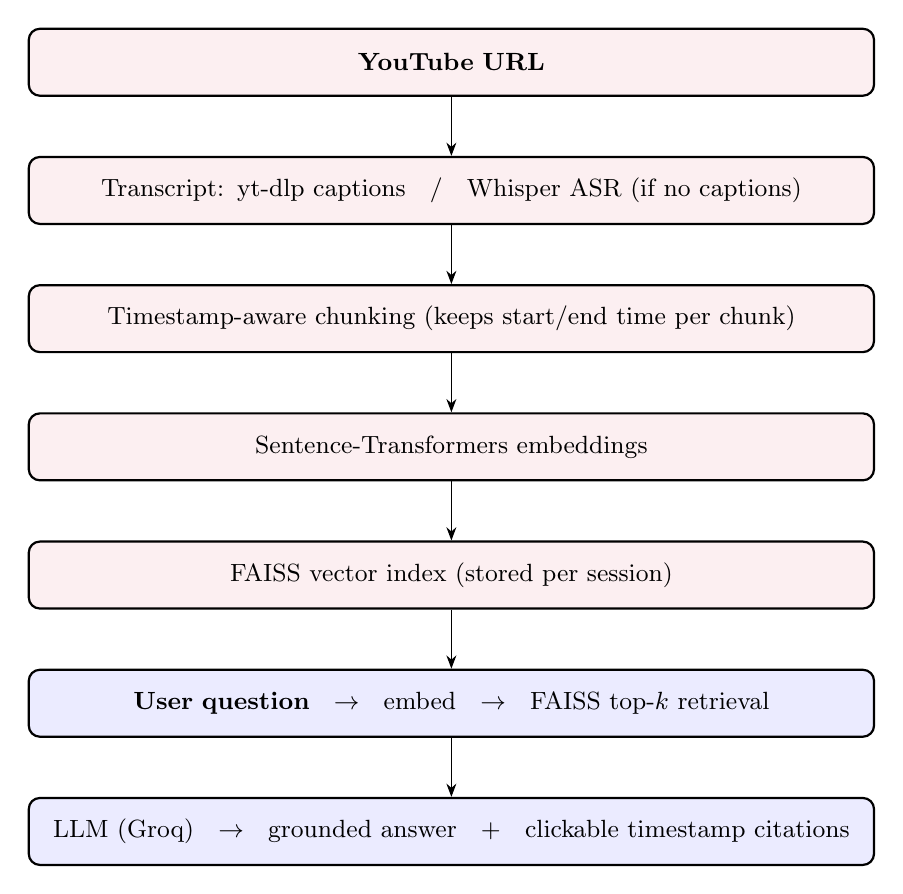
\begin{tikzpicture}[node distance=0.75cm, every node/.style={font=\small}]
  \tikzset{box/.style={draw, rounded corners, align=center, minimum height=0.85cm,
           text width=10.5cm, fill=accent!8, thick}}
  \tikzset{qbox/.style={draw, rounded corners, align=center, minimum height=0.85cm,
           text width=10.5cm, fill=blue!8, thick}}
  \node[box] (url)    {\textbf{YouTube URL}};
  \node[box, below=of url]    (tr) {Transcript: yt-dlp captions \; / \; Whisper ASR (if no captions)};
  \node[box, below=of tr]     (ch) {Timestamp-aware chunking (keeps start/end time per chunk)};
  \node[box, below=of ch]     (emb){Sentence-Transformers embeddings};
  \node[box, below=of emb]    (idx){FAISS vector index (stored per session)};
  \node[qbox, below=of idx]   (q)  {\textbf{User question} \; $\rightarrow$ \; embed \; $\rightarrow$ \; FAISS top-$k$ retrieval};
  \node[qbox, below=of q]     (ans){LLM (Groq) \; $\rightarrow$ \; grounded answer \; + \; clickable timestamp citations};
  \draw[-{Stealth}] (url)--(tr);
  \draw[-{Stealth}] (tr)--(ch);
  \draw[-{Stealth}] (ch)--(emb);
  \draw[-{Stealth}] (emb)--(idx);
  \draw[-{Stealth}] (idx)--(q);
  \draw[-{Stealth}] (q)--(ans);
\end{tikzpicture}
\caption{The ClipMind RAG pipeline. Pink boxes form the one-time ingestion phase;
blue boxes form the per-question query phase.}
\end{figure}

%====================== IMPLEMENTATION ======================
\section{Implementation}

\subsection{Backend Modules}
\begin{table}[h]
\centering
\renewcommand{\arraystretch}{1.2}
\begin{tabularx}{\textwidth}{@{}l X@{}}
\toprule
\textbf{Module} & \textbf{Responsibility} \\
\midrule
\code{config.py}        & Settings loaded from \code{.env} (provider, models, chunking parameters). \\
\code{ingest.py}        & Fetch metadata and transcript (captions first, Whisper fallback). \\
\code{chunking.py}      & Group transcript segments into overlapping, timestamped chunks. \\
\code{embeddings.py}    & Encode chunks with Sentence-Transformers. \\
\code{vector\_store.py}  & Build and search the FAISS index. \\
\code{retriever.py}     & Top-$k$ retrieval and context assembly for generation. \\
\code{llm\_client.py}    & Provider-agnostic LLM calls: answering, summary, chapters, notes, quiz, keywords, entities. \\
\code{store.py}         & In-memory per-session document store. \\
\code{schemas.py}       & Pydantic request/response models. \\
\code{routes.py}        & FastAPI route handlers. \\
\code{main.py}          & Application entry point, CORS and error handling. \\
\bottomrule
\end{tabularx}
\caption{Backend module responsibilities}
\end{table}

\subsection{Transcript Ingestion}
To keep processing fast and free, ClipMind prefers a video's existing captions, obtained
through \code{yt-dlp} (parsed from the \code{json3} caption format) with
\code{youtube-transcript-api} as a secondary source. Only when a video has no captions
does it transcribe the audio with Whisper --- using the Groq Whisper API for speed, with
a local \code{faster-whisper} model as an offline fallback. A captioned one-hour lecture
is processed in a few seconds, versus minutes for local transcription.

\subsection{Timestamp-Aware Chunking}
The transcript arrives as short timed segments. These are merged into larger overlapping
chunks suitable for retrieval, while preserving the start and end time of each chunk so
that any retrieved passage can be cited back to an exact moment in the video.

\begin{lstlisting}[language=Python, caption={Timestamp-aware chunking (abridged)}]
def build_chunks(segments, chunk_size=1000, overlap=150):
    chunks, window, length = [], [], 0
    for seg in segments:
        if window and length + len(seg["text"]) > chunk_size:
            chunks.append(_make_chunk(window))       # keeps start/end time
            window, length = _carry_overlap(window, overlap), 0
        window.append(seg); length += len(seg["text"]) + 1
    if window:
        chunks.append(_make_chunk(window))
    return chunks   # each: {"text": ..., "start": <sec>, "end": <sec>}
\end{lstlisting}

\subsection{Embeddings and Retrieval}
Each chunk is encoded into a normalised vector with the \code{all-MiniLM-L6-v2}
Sentence-Transformers model and stored in a FAISS \code{IndexFlatIP} index; because the
vectors are normalised, inner product is equivalent to cosine similarity. At query time
the question is embedded and the top-$k$ most similar chunks are retrieved.

\begin{lstlisting}[language=Python, caption={Top-$k$ retrieval (abridged)}]
def retrieve_top_k(doc_id, query, top_k=5):
    session = get_document(doc_id)
    q = embed_texts([query])[0]
    scores, idx = search(session.index, q, top_k)   # FAISS cosine search
    return [{"text": session.chunks[i]["text"],
             "start": session.chunks[i]["start"],
             "score": float(s)} for s, i in zip(scores, idx) if i != -1]
\end{lstlisting}

\subsection{Grounded Answering}
The retrieved chunks, each prefixed with its timestamp, are supplied to the LLM, which is
instructed to answer \emph{only} from the provided context and to cite the timestamps it
uses. This grounding is what prevents hallucination and enables clickable citations.

\begin{lstlisting}[language=Python, caption={Answer prompt with timestamp grounding (abridged)}]
context = "\n\n".join(f"[{fmt(c['start'])}] {c['text']}" for c in chunks)
messages = [
  {"role": "system", "content":
     "Answer using ONLY the transcript excerpts. Cite the timestamp(s) you use, "
     "e.g. (12:34). If the answer is not in the transcript, say so."},
  {"role": "user", "content": f"Excerpts:\n{context}\n\nQuestion: {question}"},
]
\end{lstlisting}

\subsection{Study-Aid Generation}
Beyond question answering, the LLM produces a structured summary, automatic chapters
(with start times), exam-style study notes, a multiple-choice quiz, keywords and named
entities, each from an appropriately assembled view of the transcript. Responses that must
be machine-readable (chapters, quiz, keywords, entities) are requested in strict JSON and
validated on the server.

\subsection{Frontend}
The React application embeds the YouTube player (via \code{react-youtube}) alongside a
tabbed workspace (Summary, Chat, Chapters, Notes, Quiz, Keywords, Entities, Transcript).
Timestamps shown anywhere in the interface are rendered as buttons; clicking one seeks the
player to that moment, tightly coupling the generated insights with the source video.

%====================== API ======================
\section{API Reference}

\begin{table}[h]
\centering
\renewcommand{\arraystretch}{1.25}
\begin{tabularx}{\textwidth}{@{}l l X@{}}
\toprule
\textbf{Method} & \textbf{Endpoint} & \textbf{Description} \\
\midrule
GET  & \code{/api/health}              & Service status and configured model. \\
POST & \code{/api/process}             & Ingest a video: transcribe, chunk, embed and index. \\
POST & \code{/api/ask}                 & Answer a question with retrieved context and citations. \\
POST & \code{/api/summary}             & Generate a structured summary. \\
POST & \code{/api/chapters}            & Generate timestamped chapters. \\
POST & \code{/api/notes}               & Generate study notes. \\
POST & \code{/api/quiz}                & Generate a multiple-choice quiz. \\
POST & \code{/api/keywords}            & Extract key concepts. \\
POST & \code{/api/entities}            & Extract named entities. \\
GET  & \code{/api/transcript/\{id\}}    & Return the full timestamped transcript. \\
\bottomrule
\end{tabularx}
\caption{REST API endpoints}
\end{table}

%====================== FEATURES ======================
\section{Features}
\begin{itemize}[leftmargin=1.4em]
  \item \textbf{Chat with the video}: natural-language Q\&A grounded in the transcript,
        with clickable timestamp citations.
  \item \textbf{Smart summary} of the whole lecture.
  \item \textbf{Automatic chapters} that split the video into clickable sections.
  \item \textbf{Study notes} and an auto-generated \textbf{multiple-choice quiz}.
  \item \textbf{Keywords} and \textbf{named entities} extracted from the content.
  \item \textbf{Searchable transcript}; click any line to jump in the video.
  \item \textbf{Captions-first ingestion} with an automatic Whisper fallback.
\end{itemize}

%====================== TESTING ======================
\section{Testing and Results}
The pipeline was tested end-to-end on real lectures:
\begin{itemize}[leftmargin=1.4em]
  \item A captioned lecture was ingested in roughly ten seconds, compared with several
        minutes when transcription had to be performed locally on the CPU --- confirming
        the value of the captions-first strategy.
  \item For a video without captions, the Groq Whisper API transcribed a 19-minute
        lecture in about 27 seconds (versus over four minutes for local transcription).
  \item Question answering returned concise, correct responses with timestamp citations;
        clicking a citation sought the embedded player to the referenced moment.
  \item Summary, chapters, notes, quiz, keywords and entities were all generated correctly
        from the indexed transcript.
\end{itemize}

\subsection*{Screenshots}
Add your own screenshots here (run the app, capture the screens, place the images next to
this report). Example usage:
\begin{lstlisting}[numbers=none]
\begin{figure}[h]
  \centering
  \includegraphics[width=0.85\textwidth]{clipmind_chat.png}
  \caption{Chatting with a lecture; answers cite clickable timestamps}
\end{figure}
\end{lstlisting}

%====================== LIMITATIONS ======================
\section{Limitations}
\begin{itemize}[leftmargin=1.4em]
  \item Indexes are held in memory and are lost when the backend restarts.
  \item The system requires an internet connection and an API key for the chosen provider.
  \item Caption availability and quality vary across videos; transcription of long videos
        without captions is slower and uses the fallback path.
  \item Free API tiers are subject to rate limits.
\end{itemize}

%====================== FUTURE SCOPE ======================
\section{Future Scope}
\begin{itemize}[leftmargin=1.4em]
  \item Multi-video and full-playlist (whole-course) question answering.
  \item A persistent vector database so processed videos are retained across sessions.
  \item Speaker diarization (attributing transcript segments to speakers).
  \item Multi-language transcripts, translation and localisation.
  \item One-click export of notes and summaries to PDF.
  \item User accounts with saved videos and study history.
\end{itemize}

%====================== CONCLUSION ======================
\section{Conclusion}
ClipMind demonstrates how Retrieval-Augmented Generation can transform a passive video
lecture into an interactive, trustworthy study companion. By combining captions-first
transcription, timestamp-aware chunking, vector retrieval and source-grounded generation,
it answers questions and produces study material that always point back to the original
video. Its provider-agnostic, dependency-light architecture keeps it fast and inexpensive,
and provides a solid foundation for the extensions outlined above.

%====================== REFERENCES ======================
\begin{thebibliography}{9}
\bibitem{reimers} Reimers, N. and Gurevych, I. \textit{Sentence-BERT: Sentence Embeddings
  using Siamese BERT-Networks}. EMNLP, 2019.
\bibitem{faiss} Johnson, J., Douze, M. and J\'egou, H. \textit{Billion-scale similarity
  search with GPUs} (FAISS). IEEE Transactions on Big Data, 2019.
\bibitem{whisper} Radford, A. et al. \textit{Robust Speech Recognition via Large-Scale
  Weak Supervision} (Whisper). OpenAI, 2022.
\bibitem{fastapi} FastAPI Documentation. \url{https://fastapi.tiangolo.com/}
\bibitem{react} React Documentation. \url{https://react.dev/}
\bibitem{groq} Groq API Documentation. \url{https://console.groq.com/docs}
\bibitem{ytdlp} yt-dlp. \url{https://github.com/yt-dlp/yt-dlp}
\end{thebibliography}

\end{document}
